%!TEX root = ../dokumentation.tex

\section{Task Modeling}
Nach Abschluss der Benutzermodellierung ging es darum, sich mit den vorhandenen Aufgaben der Anwender zu beschäftigen. Das bedeutet, sie zu identifizieren, die Struktur zu verstehen und die Beziehungen der einzelnen Aufgaben in einem konkreten Zusammenhang zu bringen.\\

Die Mensch Computer Interaktion bietet im Bereich der Aufgabenmodellierung unterschiedlichste Methodiken an, die entsprechend der Modellierungsziele und des Vorgehensmodells abgewogen wurden. Im usage centered Design wird dieser Aufgabenbereich als Task Modeling bezeichnet und setzt sich aus der Entwicklung von essential use cases mit zugehöriger use case map zusammen.\\
Wie an vorheriger Stelle erläutert, sieht das Konzept des usage centered Design vor, die Modelle auf einer abstrakteren Ebene zu entwickeln, da der allgemeinere Fokus sich nicht in Details verirrt und zu viele Abhängigkeiten formuliert. Der Vorteil für das Projekt besteht darin, dass sich erarbeitet Aufgabenstrukturen nicht zu sehr an technische Details verhaften und damit bei Rückfällen oder Änderungen der Systemstruktur weiterhin benutzbar bleiben. \\
Ein Ansatz der Aufgabenmodellierung ist das szenarienbasierte Vorgehen, bei dem durch die Entwicklung konkreter Szenarien einzelne Interaktionssbeispiele nachvollziehbar dargestellt werden. Dies eignet besonders dann, wenn der Fokus auf den Benutzer liegt und beschrieben wird, wie und warum sie mit dem System agieren. Speziell im user centered Design ist diese Methode von relevanz, spielt aber in geplantem Vorgehensmodell keine konkretere Rolle.\\

Zur Darlegung der Aufgabenstrukturen gibt es unterschiedliche Darstellungsarten. Die Hierarchical Task Analysis eignet sich gerade bei komplexen Aufgaben, da kognitive Entscheidungen nachvollziehbar dargestellt sind. Ein ähnlicher Ansatz, der meist am Anfang der Aufgabenmodellierung erfolgt, ist die Entwicklung von Work Breakdown Charts, welche einzelne Aufgabenstufen durch hierachische Zusammenhänge veranschaulichen. In Bezug auf die anfängliche Anforderungsanalyse\footnote{Konzeptseite 24} der funktionalen Aspekte, konnte der Eindruck gewonnen werden, dass auftretende Aufgaben keine komplexeren Strukturen aufweisen, die durch eine grafische Darstellung nachvollziehbarer gemacht werden müssten. Daher wurden essential use cases als erster Methode der Aufgabenmodellierung entwickelt.

\newpage
\subsection{Essential Use Cases}
Essential use cases liefern einen groben Überblick über die Struktur der Aufgabe und ist dabei in der Formulierung frei von Annahmen und Technologiebehaftungen.\\
Orientiert am Aufbau der Beispiele in der Publikum von Constantine \& Lockwood\footnote{Constantine \& Lockwood: Software for Use S.105} wurden die funktionalen Anforderungen\footnote{Konzeptseite 34}, die zu diesem Zeitpunkt vorhanden waren, umgesetzt.
Eine Herausforderung stellte dabei die Wahl einer geeigneten Sprache und der Detailierungsgrad dar. Daher wurden sie innerhalb des Projektzeitraums mehrfach überarbeitet und erweitert. Im weiteren Verlauf der ersten Iterationsphase der MCI Auseinandersetzung, führte die Evaluation des ersten abstract prototype (wird im nächsten Kapitel 2.4 genauer beschrieben), dazu, dass die vorhandenen essential use cases einer erneuten Überarbeitung unterzogen werden mussten, da sie nicht alle (bis dahin) funktionalen Aspekte berücksichtigten.\\

Im Folgenden sind die erarbeiteten use cases dargestellt. Diese Übersicht stellt dabei noch keine Gewährleistung auf letztendliche Vollständigkeit dar, da im späteren Projektverlauf neue Anforderungen erkannt wurden, die aus zeitlichen Gründen keiner weiteren Iterationsphase unterstanden.\\ 
Rückblickend betrachtet konnte an dieser Stelle festgestellt werden, dass die use cases "wähleAktion" und "userAusloggen" eher elementare Funktionen der Anwendung sind keine konkreten Anforderungen, die sich aus der speziellen Domäne ergeben. In einer weiteren Überarbeitung könnten sie daher vernachlässigt werden.

\newpage
Essential Use Case \#1 (Tabelle \ref{tab:registrieren}) sieht die Registrierung eines Anwenders vor, welcher beim erstmaligen Start der Anwendung ein Benutzeraccount anlegen muss.
\begin{table}[H]
\caption{Essential Use Case \#1 registriereUser }
\centering
\begin{tabular}{l l}
\\ [-0.5ex]

\hline\hline
\\ [-0.5ex]
user intention & system responsibility
\\ [1.5ex]
\hline
\\ [-0.5ex]
Registrierung initiieren            &                                \\[1ex]
                              & Aktion anbieten und bei Wahl ausführen  \\[1ex]
Userinformationen angeben           &                                \\[1ex] 
                              & Userinformationen aufnehmen          \\[1ex]
                              & Userinformationen präsentieren       \\[1ex]
eingegebene Informationen bestätigen   &                                \\[1ex]
                              & Bestätigung abfragen, bei Auswahl akzeptieren  \\[1ex]
                              & Registrierung durchführen, Aktion beenden  \\[1ex]


\hline
\end{tabular}
\label{tab:registrieren}
\end{table}

\newpage
Essential Use Case \#2 (Tabelle \ref{tab:profilverwalten}) befasst sich mit dem Anwenderziel, sein bereits angelegtes Profil zu verwalten, indem angegeben Funktionen geändert oder das Profil gelöscht wird.
\begin{table}[H]
\caption{Essential Use Case \#2 verwalteProfil }
\centering
\begin{tabular}{l l}
\\ [-0.5ex]

\hline\hline
\\ [-0.5ex]
user intention & system responsibility
\\ [1.5ex]
\hline
\\ [-0.5ex]
Verwaltung initiieren      &                                 \\[1ex]
                     & Aktion anbieten und bei Wahl ausführen     \\[1ex]
Profilart wählen        &                                 \\[1ex]
                     & Auswahl anbieten und bei Wahl ausführen  \\[1ex]             
vorhandene Informationen   &                                 \\[1ex]
angezeigt bekommen         &                                 \\[1ex]
                     & vorhandene Informationen präsentieren      \\[1ex] 
Informationen ändern       &                                 \\[1ex] 
                     & Aufnahme neuer Informationen ermöglichen    \\[1ex]
                     & löschen des Profils ermöglichen          \\[1ex]
Änderungen bestätigen      &                                 \\[1ex]
                     & Bestätigung anbieten, bei Wahl ausführen   \\[1ex]
                     & neue Informationen sichern, Aktion beenden \\[1ex]

\hline
\end{tabular}
\label{tab:profilverwalten}
\end{table}

\newpage
Essential Use Case \#3 (Tabelle \ref{tab:reiseprofil}) beschreibt die Erstellung eines "Reiseprofils". Im Rahmen des Projektes wurde diese Bezeichnung dafür vergeben, wenn der Reisende für eine Suchanfrage die gewünschte Ausstattung des Grundstückes und relevante Informationen zur Gruppengröße, Reisezeit und Preisvorstellung angibt.
\begin{table}[H]
\caption{Essential Use Case \#3 erstelleReiseprofil }
\centering
\begin{tabular}{l l}
\\ [-0.5ex]

\hline\hline
\\ [-0.5ex]
user intention & system responsibility
\\ [1.5ex]
\hline
\\ [-0.5ex]
Erstellung initiieren      &                                 \\[1ex]
                     & Aktion anbieten und bei Wahl ausführen   \\[1ex]
Reiseinformationen anlegen    &                                 \\[1ex] 
                     & neue Reiseinformationen aufnehmen        \\[1ex]
                     & Reiseinformationen präsentieren          \\[1ex]
eingegebene Informationen bestätigen   &                                 \\[1ex]
                     & Bestätigung anbieten, bei Wahl akzeptieren \\[1ex]
                     & Reiseprofil sichern, Aktion beenden      \\[1ex]

\hline
\end{tabular}
\label{tab:reiseprofil}
\end{table}


\newpage
Essential Use Case \#4 (Tabelle \ref{tab:mietobjekt}) beschreibt die Durchführung einer neuen Suchanfrage des Reisenden, um einen passenden Unterkunftsanbieter zu finden.

\begin{table}[H]
\caption{Essential Use Case \#4 sucheMietobjekt }
\centering
\begin{tabular}{l l}
\\ [-0.5ex]

\hline\hline
\\ [-0.5ex]
user intention & system responsibility
\\ [1.5ex]
\hline
\\ [-0.5ex]
Suche initiieren        &                                 \\[1ex]
                     & Aktion anbieten und bei Wahl ausführen   \\[1ex]
Mietanfrage spezifizieren  &                                 \\[1ex]
                     & vorhandene Mietanfrage präsentieren      \\[1ex]
                     & und Option für neuen Mietanfrage anbieten  \\[1ex]
Option auswählen           &                                 \\[1ex] 
                     & gewählte Option ausführen                \\[1ex]
                     & Mietanfrage präsentieren                 \\[1ex]
Anfrage starten         &                                 \\[1ex] 
                     & Aktion ausführen und Anfrage bearbeiten  \\[1ex]
Rückmeldung erhalten    &                                 \\[1ex]
                     & Ergebnis präsentieren                 \\[1ex]
                     & weitere Aktionen anbieten                \\[1ex]


\hline
\end{tabular}
\label{tab:mietobjekt}
\end{table}

\newpage
Essential Use Case \#5 (Tabelle \ref{tab:mietanfrage}) beschreibt die Aufgabe des Vermieters, auf eine erhaltene Mietanfrage zu reagieren und sie zu anzunehmen oder abzulehnen.
\begin{table}[H]
\caption{Essential Use Case \#5 beantworteMietanfrage }
\centering
\begin{tabular}{l l}
\\ [-0.5ex]

\hline\hline
\\ [-0.5ex]
user intention & system responsibility
\\ [1.5ex]
\hline
\\ [-0.5ex]
Mietanfrage erhalten       &                                 \\[1ex]
                     & neue Mietanfrage präsentieren            \\[1ex]
Mietanfrage beantworten    &                                 \\[1ex] 
                     & Reiseprofil präsentieren              \\[1ex]
                     & Aktionen anbieten und ausführen          \\[1ex]
Rückmeldung erhalten    &                                 \\[1ex]
                     & über Ausführung informieren           \\[1ex]
                     & Aktion beenden                     \\[1ex]

\hline
\end{tabular}
\label{tab:mietanfrage}
\end{table}


\newpage
Essential Use Case \#6 (Tabelle \ref{tab:bezahlung}) stellt die Aufgabe dar, die Bezahlung eines getätigten Mietauftrages durchzuführen. Diese Aufgabe sollte spätestens vor Weiterreise geschehen.
\begin{table}[H]
\caption{Essential Use Case \#6 bezahleMiete }
\centering
\begin{tabular}{l l}
\\ [-0.5ex]

\hline\hline
\\ [-0.5ex]
user intention & system responsibility
\\ [1.5ex]
\hline
\\ [-0.5ex]
Bezahlung initiieren    &                                 \\[1ex]
                     & Aktion anbieten und bei Wahl ausführen   \\[1ex]
Mietauftrag wählen         &                                 \\[1ex] 
                     & Mietaufträge präsentieren und Wahl ermöglichen \\[1ex]
Bezahlung durchführen      &                                 \\[1ex]
                     & Auftragsinformationen präsentieren       \\[1ex]
                     & Informationsaufnahme anbieten            \\[1ex]
Auftrag bestätigen         &                                 \\[1ex]
                     & Zusammenfassung der Informationen präsentieren \\[1ex]
                     & Optionen anbieten  und ausführen         \\[1ex]
Rückmeldung erhalten    &                                       \\[1ex]
                     & Ergebnis präsentieren                  \\[1ex]
                     & weitere Aktionen anbieten                 \\[1ex]


\hline
\end{tabular}
\label{tab:bezahlung}
\end{table}


\newpage
Essential Use Case \#7 (Tabelle \ref{tab:bewertung}) beschreibt die Absicht des Benutzers, den Verleihpartner nach durchgeführtem Vermietprozess zu bewerten.
\begin{table}[H]
\caption{Essential Use Case \#7 bewerteUser }
\centering
\begin{tabular}{l l}
\\ [-0.5ex]

\hline\hline
\\ [-0.5ex]
user intention & system responsibility
\\ [1.5ex]
\hline
\\ [-0.5ex]
Bewertung initiieren    &                                 \\[1ex]
                     & Aktion anbieten und bei Wahl ausführen   \\[1ex]
Mietauftrag wählen         &                                 \\[1ex] 
                     & Mietaufträge präsentieren und Wahl ermöglichen \\[1ex]
Bewertung abgeben          &                                 \\[1ex]
                     & Bewertungsinformationen aufnehmen        \\[1ex]
                     & Aktion durchführen                 \\[1ex]
Rückmeldung erhalten    &                                 \\[1ex]
                     & Ergebnis präsentieren                    \\[1ex]
                     & Aktion beenden                     \\[1ex]

\hline
\end{tabular}
\label{tab:bewertung}
\end{table}


\newpage
Essential Use Case \#8 (Tabelle \ref{tab:kontaktaufnahme}) sieht die Kontaktaufnahme zweier Anwender vor, nachdem eine Mietanfrage erfolgreich durchgeführt und angenommen wurde. Hierbei sind Textnachrichten zur Kommunikation zwischen Vermieter und Mieter gemeint.
\begin{table}[H]
\caption{Essential Use Case \#8 kontaktiereUser }
\centering
\begin{tabular}{l l}
\\ [-0.5ex]

\hline\hline
\\ [-0.5ex]
user intention & system responsibility
\\ [1.5ex]
\hline
\\ [-0.5ex]
Kontaktaufnahme initiieren &                                 \\[1ex]
                     & Aktion anbieten und bei Wahl ausführen   \\[1ex]
relevanten Mietauftrag     &                                 \\[1ex] 
anzeigen             &                                 \\[1ex] 
                     & vorhandene Mietaufträge präsentieren        \\[1ex]
                     & gewählten Auftrag präsentieren        \\[1ex]
Nachricht verfassen        &                                 \\[1ex]
                     & Nachrichtenaufnahme anbieten             \\[1ex]
                     & Aktion durchführen                 \\[1ex]
\hline
\end{tabular}
\label{tab:kontaktaufnahme}
\end{table}


\newpage
Essential Use Case \#9 (Tabelle \ref{tab:ausloggen}) beschreibt das Ausloggen vom verbundenen Account eines Nutzers.
\begin{table}[H]
\caption{Essential Use Case \#9 userAusloggen }
\centering
\begin{tabular}{l l}
\\ [-0.5ex]

\hline\hline
\\ [-0.5ex]
user intention & system responsibility
\\ [1.5ex]
\hline
\\ [-0.5ex]
Ausloggen initiieren    &                                 \\[1ex]
                     & Aktion anbieten und bei Wahl ausführen   \\[1ex]
Rückmeldung erhalten    &                                 \\[1ex]
                     & Ergebnis präsentieren                 \\[1ex]
                     & Aktion beenden                     \\[1ex]

\hline
\end{tabular}
\label{tab:ausloggen}
\end{table}



Essential Use Case \#10 (Tabelle \ref{tab:aktionen}) beschreibt das Ziel des Anwenders, eine der vorhandenen Funktionen wie  "Suchanfrage starten" zu finden und auszuführen. Dieser use case entstand im Rahmen der letzten Überarbeitung, als Ergebnis der Auswertung des ersten abstrakten Prototypen. Die Tätigkeit die innerhalb dieses Anwendungsfall dargestellt ist, stellt den ersten Schritt jedes vorherigen use cases dar, wurde für ein weiteres content model jedoch in Betracht gezogen.

\begin{table}[H]
\caption{Essential Use Case \#10 wähleAktion }
\centering
\begin{tabular}{l l}
\\ [-0.5ex]

\hline\hline
\\ [-0.5ex]
user intention & system responsibility
\\ [1.5ex]
\hline
\\ [-0.5ex]
mögliche Aktion finden        &                                \\[1ex]
                        & vorhandene Aktionen präsentieren        \\[1ex]
Aktion ausführen           &                                \\[1ex] 
                        & Auswahl der Aktion ermöglichen       \\[1ex]
                        & Aktion initiieren                    \\[1ex]
\hline
\end{tabular}
\label{tab:aktionen}
\end{table}

\newpage
\subsection{Use Case Map}
Einige der auftretenden use cases, stehen bei der Verwendung des Systems in unmittelbarem Zusammenhang. Die Beziehung untereinander ist in der use case map in Abbildung \ref{fig:use}) gezeigt. Dieses Modell stellte für weitere Ausarbeitungen den Vorteil dar, dass beim Prototyping Verbindungen zwischen den Funktionen und den möglichen Working Spaces der Anwendung veranschaulicht werden. Bei der Umsetzung wurde deutlich, einige der use cases weiter verwenden, die zuvor jedoch nicht genauer definiert wurden. Innherhalb der Grafik wurden diese bereits mit eingebunden, da sie ein essentieller Bestandteil der jeweiligen Fälle sind.

\begin{figure}[H]
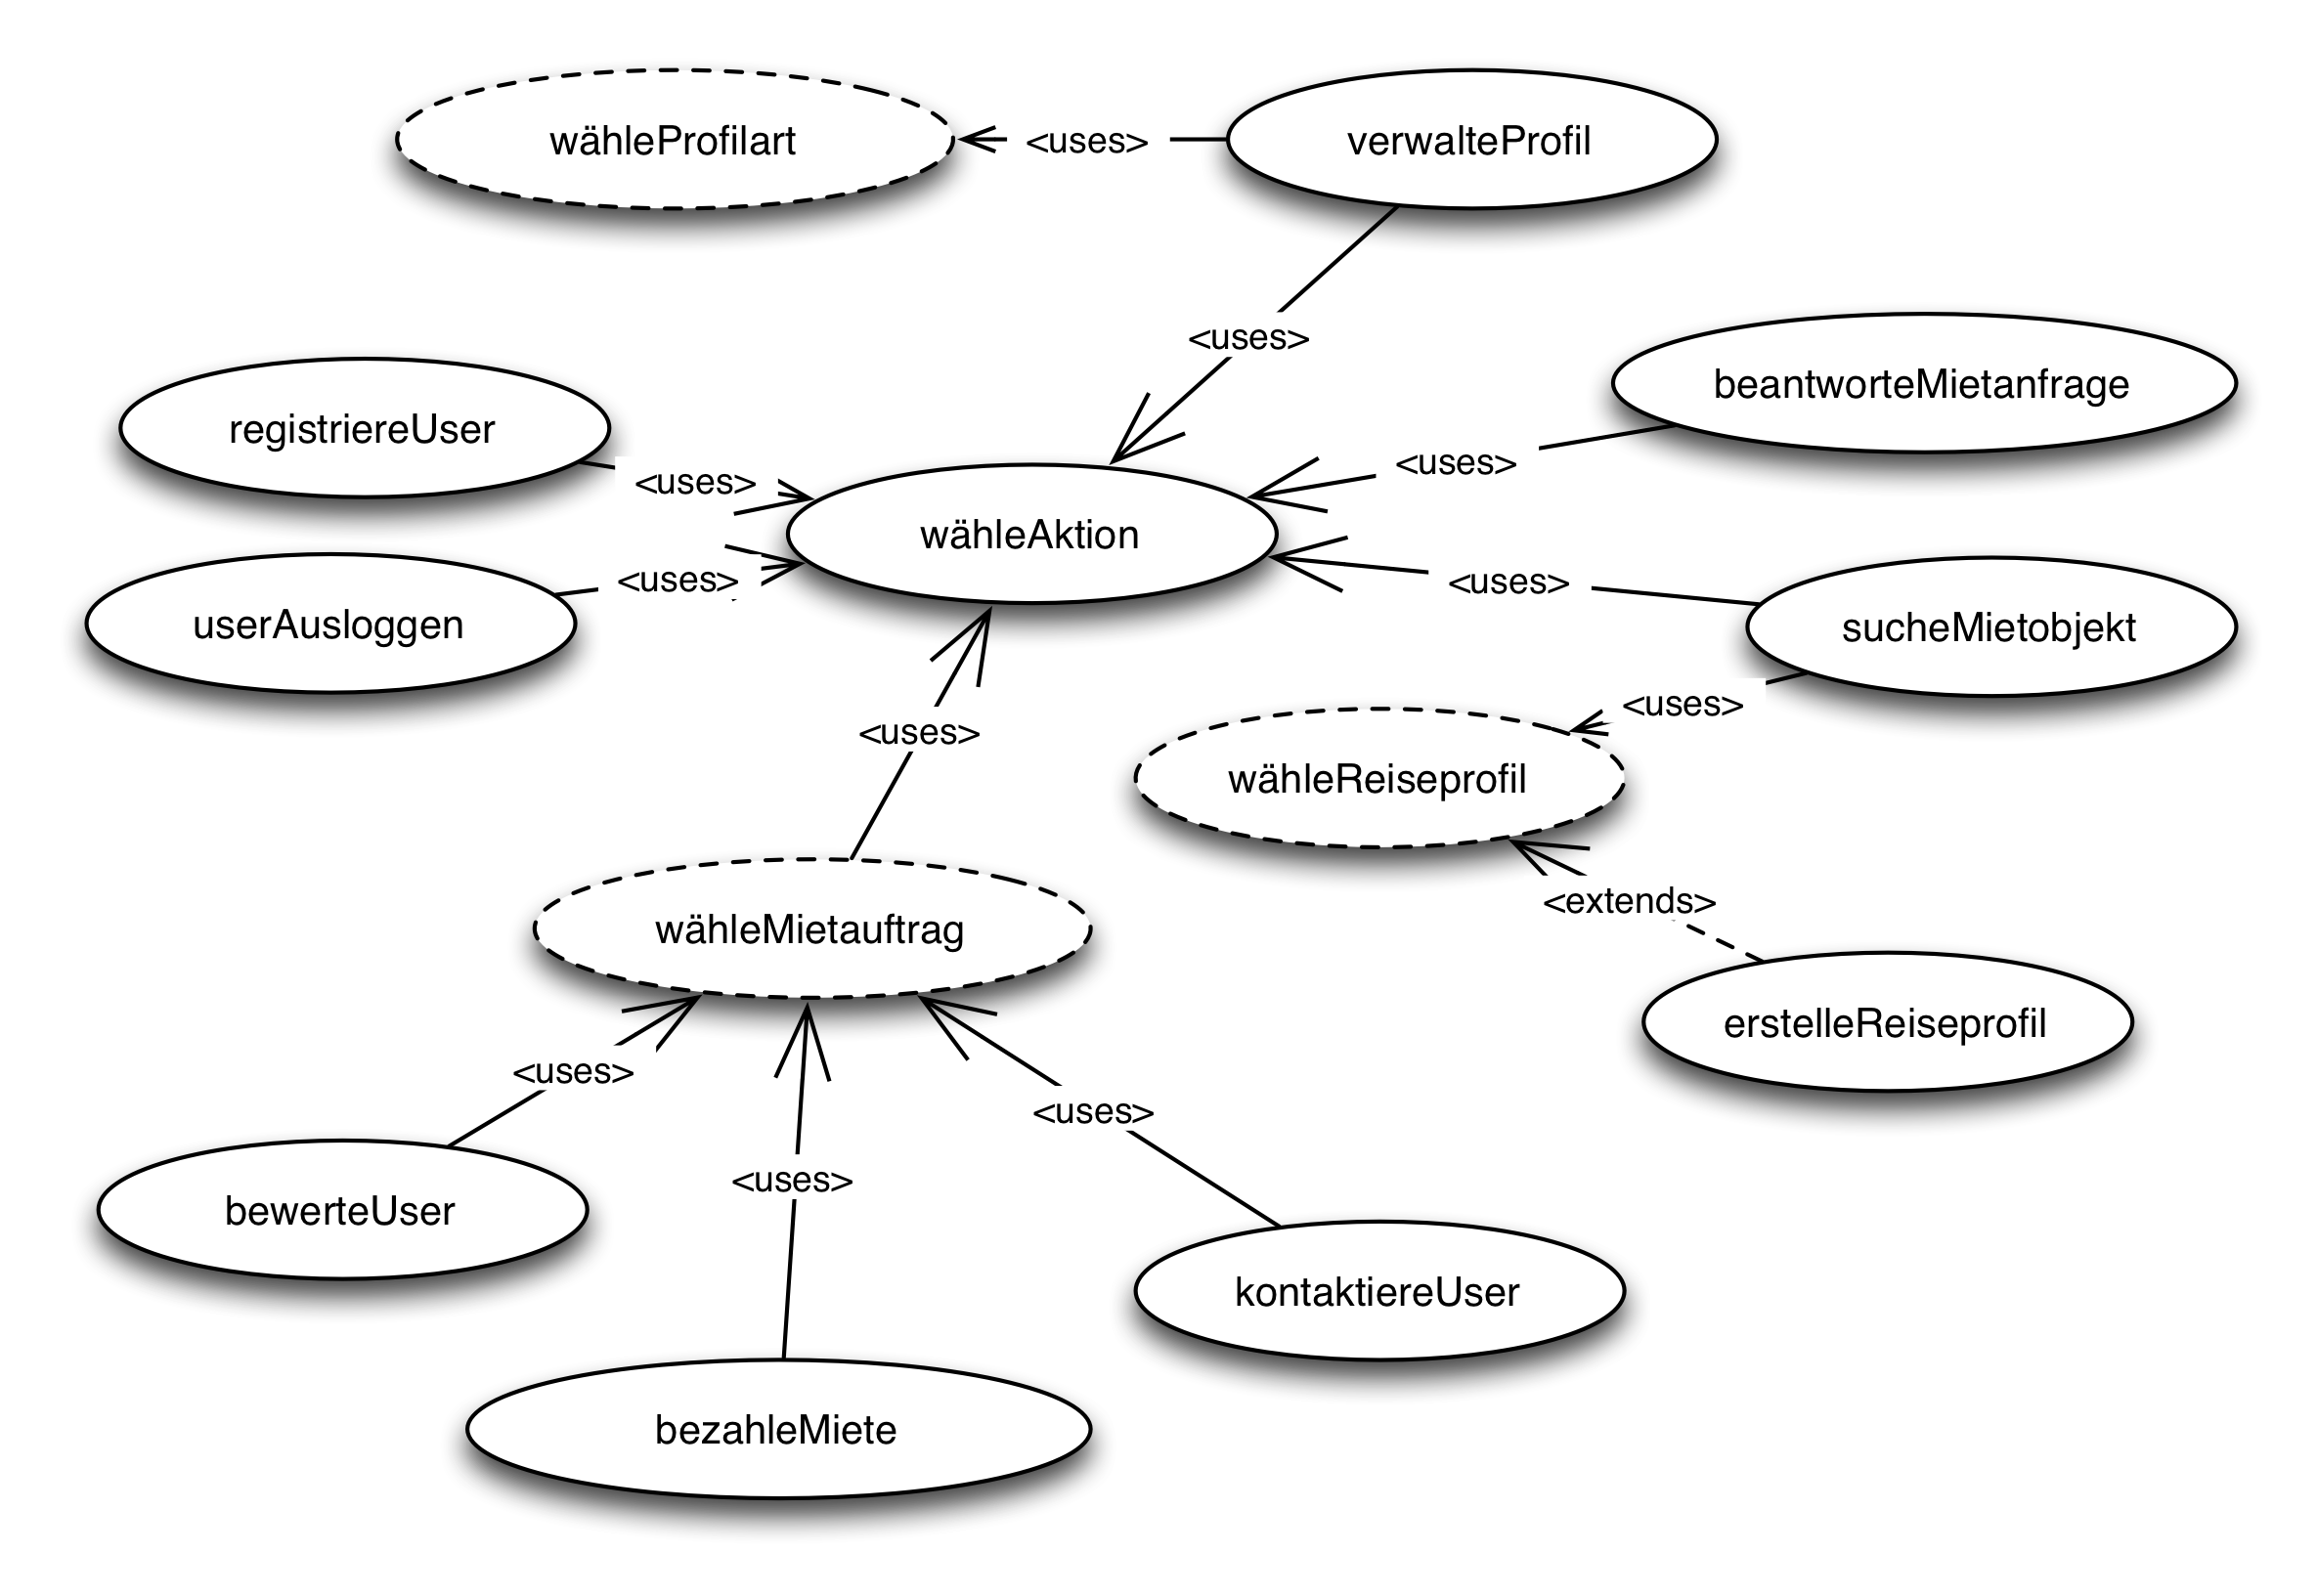
\includegraphics[width=1\textwidth]{./images/use.png}
\caption{Evaluationsprotokoll 2.2}
\label{fig:use}
\end{figure}

Da der Anwendungsfall "wähleAktion" stellvertretend die erste user intention der Anwendungsfälle ist, scheint es nicht verwunderlich das alle in verwenden. Diese Darstellung repräsentiert nach eigenen Einschätzungen noch noch keine finale Use Case Map aller vorhandenen Anwendungsfälle die im Zusammenhang mit der Anwendung auftreten können. Auch wenn viele wesentliche Aufgaben hiermit bereits erfasst wurde, wäre eine erneute Überarbeitung in einer weiteren Iterationsphase unumgänglich. Diese hat jedoch keinen Einzug in das Projekt gefunden.

\newpage
\subsection{Concrete Use Cases}
(Die Ausarbeitung der concrete use cases fand nach der Evaluation des ersten abstrakten Prototypen statt und nicht im direkten Anschluss vorheriger Methoden. Aufgrund der Thematik, wird dieser Abschnitt bereits in diesem Kapitel beschrieben.)\\

Die Evaluation des Prototypen verdeutlichte, dass zu diesem Zeitpunkt noch kein genaues Verständnis darüber gewonnen werden konnte, inwiefern die einzelnen Use Cases über mehrere Interface Contexte miteinander in Verbindung gebracht werden können, wenn Aufgaben aufeinander aufbauen. Zusätzlich dazu konnte der abstrakte Charakter nicht immer zum genauen Verständnis des Aufgabenablaufs dienen.\\
Um für komplexere Aufgaben eine bessere Übersicht der user intention und Systemreaktion zu erhalten, wurden aus den essiental use cases, concrete use cases abgeleitet. Auch hierbei stellte sich während der Ausarbeitung heraus, dass sich die genaue Beschreibung der Interaktionsschritte schwieriger gestaltet als Anfangs angenommen und dadurch einige Zeit und Versionen in Anspruch nahm. Nach einiger Arbeitszeit wurde entschlossen, diese Beschreibungstechnik vorerst ruhen zu lassen und mit den vorhandenen Ergebnissen zu arbeiten. Ein Problem was sich im Nachhinein erkennen lies, ist der starke Einbezug von Interface bezogenen Angaben. Die system responsibilty wird an einigen Stellen eventuell zu genau beschrieben, wodurch die unterschiedlichen Strukturen, durch unterschiedliche Gedanken zur Interfacegestaltung entstanden. Die Ergebnisse dieser Arbeit sind die kommenden Use Cases.



\newpage
Use Case \#1 (Tabelle \ref{tab:anmeldenUC}) zeigt die einzelnen Schritte die bei der Registrierung von einem neuen User durchgeführt werden sollten.
Nachdem der User die Korrektheit seiner Daten bestätigt, wurde in Betracht gezogen, den weiteren Use Case "Account verifizieren" durchzuführen und damit einen wesentlichen Sicherheitsaspekt des Systems einzubinden. Die Verifizierung ist im Rahmen dieses Projekt jedoch nicht genauer geplant worden und nur konzeptioneller Inhalt einer zukünftigen Iterationsphase.

\begin{table}[H]
\caption{Use Case\#1 registriereUser }
\centering
\begin{tabular}{l l}
\\ [-0.5ex]

\hline\hline
\\ [-0.5ex]
user intention & system responsibility
\\ [1.5ex]
\hline
\\ [-0.5ex]
Funktion zur Registrierung auswählen   &                                   \\[1ex]
                                       & Funktion bereitstellen, die dies    \\[1ex]
                                       & ermöglicht, über Richtlinien hinweisen       \\[1ex]

Relevante Informationen eingeben                       &                                   \\[1ex] 
Personeninformationen Name, Vorname  &                                   \\[1ex] 
Gebdat etc.   &                                   \\[1ex] 

                                       & Eingabefelder bereitstellen, Informationen    \\[1ex]
                                       & aufnehmen, weitere Schritte ermöglichen    \\[1ex]
                                       & auf Richtlinien hinweisen    \\[1ex]

Kenntnissnahme zu Richtlinien bestätigen        &                                   \\[1ex]
                                        & Bestätigung ermöglichen                 \\[1ex]
Korrektheit der Daten prüfen und bestätigen        &                                   \\[1ex]
                                       & Funktion zur Bestätigung anbieten,          \\[1ex]
                                       & Daten nach syntax prüfen, ggf.  \\[1ex]
                                       & Rückmeldung, Userdaten an Serveranwendung \\[1ex]
                                       & senden und speichern  \\[1ex]
                                       & weiterleiten zum Hauptcontext \\[1ex]
\hline
\end{tabular}
\label{tab:anmeldenUC}
\end{table}

\newpage

Use Case \#2 (Tabelle \ref{tab:profilbearbeitenUC}) beschreibt das Verwalten eines bereits vorhandenen Benutzerprofils.
\begin{table}[H]
\caption{Use Case\#2 verwalteBenutzerprofil }
\centering
\begin{tabular}{l l}
\\ [-0.5ex]

\hline\hline
\\ [-0.5ex]
user intention & system responsibility
\\ [1.5ex]
\hline
\\ [-0.5ex]
Funktion zur Verwaltung auswählen   &                                      \\[1ex]
                                    & Funktion anbieten und bei Bestätigung      \\[1ex]
                                    & Context wechseln      \\[1ex]

Bisherige Angaben einsehen          &                                      \\[1ex]
                                    & gespeicherte Informationen anzeigen   \\[1ex]
                                    & Funktion zur Überarbeitung bereitstellen  \\[1ex] 
Neuen Informationen eingeben        &                                      \\[1ex] 
                                    & Eingabemöglichkeit anbieten,  \\[1ex]
                                    & überschreiben der vorhanden Informationen   \\[1ex]
                                    & Funktion zum speichern anbieten \\[1ex]
Neue Informationen abspeichern      &                                      \\[1ex]
                                    & Funktion zum abspeichern anbieten             \\[1ex]
                                    & nach Erfolg Rückmeldung dazu    \\[1ex]
\hline
\end{tabular}
\label{tab:profilbearbeitenUC}
\end{table}

\newpage
Use Case \#3 (Tabelle \ref{tab:mietauftragUC}) beschreibt das Erstellen eines Reiseprofils. Im Laufe des Projektes hat sich dieser Anwendungsfall leicht verändert, soll in dieser Form aber nicht ausgeschlossen werden. Das Speichern des Reiseprofils unterstützt den Anwender darin, häufig auftretenden Eingaben zu vermeiden. Die Implementation im abgegeben Prototypen, weicht in den letzten Schritten von der hier dargestellten Form ab.
\begin{table}[H]
\caption{Use Case\#3 erstelleReiseprofil }
\centering
\begin{tabular}{l l}
\\ [-0.5ex]

\hline\hline
\\ [-0.5ex]
user intention & system responsibility
\\ [1.5ex]
\hline
\\ [-0.5ex]
Funktion zum neuen Mietauftrag wählen     &                                   \\[1ex]
                                 & Funktion bereitstellen, die dies ermöglicht   \\[1ex]
Organisatorische Informationen & \\[1ex]
wie Preis, Ort und Gruppe eintragen  &                                   \\[1ex] 
                                          & Eingabefelder bereitstellen und            \\[1ex]
                                          & Informationen aufnehmen                 \\[1ex]
                                          & Dialog informiert über benötigte \\[1ex]
                                          & Informationen \\[1ex]
Gewünschte Austattung auswählen           &                                   \\[1ex]
                                          & Austattungsmerkmale anzeigen und           \\[1ex]
                                         & Auswahl über Menü ermöglichen           \\[1ex]
Informationen bestätigen und abspeichern  &                                   \\[1ex]
                                          & Funktion zum abspeichern anbieten          \\[1ex]
                                          & (Alternativ Suchanfrage starten))         \\[1ex]
\hline
\end{tabular}
\label{tab:mietauftragUC}
\end{table}

\newpage
Use Case \#4 (Tabelle \ref{tab:mietobjektUC}) beschreibt das Durchführen einer neuen Suchanfrage des Reisenden.
\begin{table}[H]
\caption{Use Case\#4 findeMietobjekt }
\centering
\begin{tabular}{l l}
\\ [-0.5ex]

\hline\hline
\\ [-0.5ex]
user intention & system responsibility
\\ [1.5ex]
\hline
\\ [-0.5ex]
Funktion zur neuen Suchanfrage starten    &                                   \\[1ex]
                              & Funktion bereitstellen, die dies ermöglicht   \\[1ex]
Passenden Mietauftrag zur Reise wählen &                                   \\[1ex]
                              & Vorhandene Mietaufträge anzeigen \\[1ex]
                              & und Auswahl ermöglichen, Option zum anlegen   \\[1ex]
                              & eines neuen Auftrags anzeigen              \\[1ex]
Suchanfrage ausführen               &                                   \\[1ex] 
                              & Ausgewählten Auftrag anzeigen  und Suchanfrage   \\[1ex]
                              & funktional ermöglichen, nach vollständiger      \\[1ex]
                              & Angabe relevanter Informationen \\[1ex]
                              & Anfrage weiterleiten. \\[1ex]
                              & Benutzer über getätigte Suche informieren     \\[1ex]
Rückmeldung zu vorhandenen Angeboten   &                                   \\[1ex]
erhalten                      &                                   \\[1ex]
                              & Wenn kein Angebot vorhanden ist, direkte      \\[1ex]
                              & Rückmeldung. Ansonsten Abfrage    \\[1ex]
                              & an Server, ob Vermieter angenommen hat.    \\[1ex]
                              & Meldung an Benutzer schicken bei Treffer      \\[1ex]
                              & nach Ablauf einer kritischen Zeit.            \\[1ex]
\hline
\end{tabular}
\label{tab:mietobjektUC}
\end{table}

\newpage
Use Case \#5 (Tabelle \ref{tab:mietanfrageUC}) stellt den Fall dar, dass ein Grundstückbesitzer über eine Anfrage informiert wird und anschließend darauf reagiert.
\begin{table}[H]
\caption{Use Case\#5 beantworteMietanfrage }
\centering
\begin{tabular}{l l}
\\ [-0.5ex]

\hline\hline
\\ [-0.5ex]
user intention & system responsibility
\\ [1.5ex]
\hline
\\ [-0.5ex]
Meldung über relevante Mietanfrage  &                                   \\[1ex]
erhalten                             &                                   \\[1ex]
                                     & Mietauftrag empfangen und lokal matchen    \\[1ex]
                                    & bei Bestätigung Meldung mit Informationen     \\[1ex]
                                    & auf dem Display hervorheben, Benachrichtigen  \\[1ex]
Mieterdaten ansehen               &                                   \\[1ex]
                                  & Reisedaten anzeigen: Datum Gruppengröße    \\[1ex]
                                   & Preisvorstellung, Anfragezeit              \\[1ex]
Mietanfrage beantworten            &                                   \\[1ex] 
                                   & Funktion anbieten zur Annahme oder Ablehnung  \\[1ex]
                                   & der Anfrage, Meldung an Mieter schicken       \\[1ex]
Annahme des Auftrags erhalten      &                                   \\[1ex]
                                   & Bestätigung des Mieters empfangen, Auswahl \\[1ex]
                                   & dem Vermieter anzeigen und ggf. weitere       \\[1ex]
                                   & Funktion zum Senden der Objektinformationen   \\[1ex]
Objektinformationen verschicken     &                                   \\[1ex]
                  &      Funktionsausführung                             \\[1ex]



\hline
\end{tabular}
\label{tab:mietanfrageUC}
\end{table}


\newpage
Use Case \#6 (Tabelle \ref{tab:mietobjektAUC}) beschreibt den Anwendungsfall, wenn ein angemeldeter Benutzer ein neues Grundstück anlegen will, dass er zur Vermietung anbietet.

\begin{table}[H]
\caption{Use Case\#6 registriereMietobjekt }
\centering
\begin{tabular}{l l}
\\ [-0.5ex]

\hline\hline
\\ [-0.5ex]
user intention & system responsibility
\\ [1.5ex]
\hline
\\ [-0.5ex]
Funktion zur Mietobjektverwaltung auswählen      &                                   \\[1ex]
                                        & Funktion bereitstellen, die dies ermöglicht   \\[1ex]
Auswahl ob altes Objekt bearbeiten oder      &                                   \\[1ex]
neues Anlegen                                 &                                   \\[1ex]
                                               & Funktion bereitstellen, die dies ermöglicht   \\[1ex]
Neues Mietobjekt registrieren                    &                                   \\[1ex] 
Besitzer festlegen                          &                                   \\[1ex] 
                                           & Verifizierung des Besitzers durch Accountdaten \\[1ex]
                                          & Eingabefelder bereitstellen und prüfen     \\[1ex]
Objektstandort angeben                  &                                   \\[1ex]
                                              & Funktion zur Standortbestimmung bereitstellen  \\[1ex] 
                                          &  Prüfung ob Ort von Anwendung erkannt             \\[1ex]   

Objektmerkmale wie Größe, Preis eingeben  &                                   \\[1ex]
                                           & Eingabefelder anzeigen und Eingabe über       \\[1ex]
                                           & vordefinierte Optionen ermöglichen         \\[1ex]
angebotene Austattung angeben           &                                   \\[1ex]
                                           & Austattungsmerkmale anzeigen und           \\[1ex]
                                            & Auswahl über Menü ermöglichen           \\[1ex]
Informationen kontrollieren, bearbeiten   &                                   \\[1ex]
und abspeichern                           &                                   \\[1ex]
                                          & Syntaxcheck  \\[1ex]
                                          & eingegebene Daten anzeigen und lokal  \\[1ex]
                                          & speichern; Zuordnung Mieter,    \\[1ex]
                                          & Ort und Objekt an Serveranwendung\\[1ex]



\hline
\end{tabular}
\label{tab:mietobjektAUC}
\end{table}

\newpage
\subsubsection{Szenarienentwicklung}
Use cases spiegeln die Aufgabenstruktur von Tätigkeiten wieder, die prinzipiell nach einem ähnlichen Schema verlaufen. Betrachtet man einen use case als Klasse, so kann eine konkrete Instanz dafür in Form eines Szenarios beschrieben werden. (Keine allgemeingültige Ansicht der MCI)\\ Bei der Planung der Benutzermodellierung wurde die bewusste Entscheidung getroffen, Personae für spätere Methoden zu erarbeiten, um vielseitige Verhaltensweisen und Ansichten zur Problemdomäne zu durchdenken.\footnote{Beschrieben in Kapitel 2.2 Seite 5} Dieser Ansatz erschien in sofern sinnvoll, das unterschiedliche Nutzungsmotivationen bedacht werden und somit neue Anforderungen gewonnen werden könnten. In der Konzeptphase fand die Auseinandersetzung mit Risiken statt\footnote{Konzeptseite 10}, bei der ein wesentliches Risiko der Nutzerzuspruch war. Haben die Anwender kein Interesse an der Anwendung oder fühlen sich nicht ausreichend unterstützt, werden sie das System meiden und der Erfolg ist stark gefährdet. Um für solche Fälle mögliche Schwachstellen zu entdecken, war die Erarbeitung von Szenarien als zusätzliche Bearbeitung angedacht.\\
Aus zeitlichen Gründen wurde diese Modellierungstiefe dann letztendlich doch nicht erreicht, da sie für das geplante Ziel keine direkte Notwendigkeit zeigten. Die Szenarien wären aufgrund ihrerer Detailierung für einen späteren Designprozess ungeeignet gewesen und die Ergebnisse hätten keinen projektrelevanten Mehrwert geboten. Das grundsätzliche Vorgehen basiert auf der Analyse der Interaktionsschritte und Aufgabenstrukturen und nicht darauf, wie einzelne Anwender speziell darauf reagieren.






